\chapter{Nomogrami in posplošeni linearni modeli}

Na področju odkrivanja znanj iz podatkov gradimo modele, ki jih je treba -- z namenom razumevanja odkritih vzorcev -- ustrezno predstaviti uporabniku. Eden najučinkovitejših načinov predstavitve je grafični, saj lahko v dvodimenzionalnih vizualizacijah preprosto primerjamo vpliv (moč) različnih dejavnikov in njihove medsebojne interakcije. V preteklih poglavjih smo grafične predstavitve uporabljali predvsem za prikaz podatkovnih primerov, ne pa samih modelov, v tem poglavju pa se osredotočamo prav na grafične prikaze modelov. Pri tem se bomo omejili na modele, pri katerih so vhodne značilke med seboj linearno povezane, ter na posebno obliko njihove predstavitve, imenovano nomogrami. \marginnote{Beseda {\em nomogram} izhaja iz grških besed {\em nomos} (zakon) in {\em gramme} (črta) ter označuje grafični prikaz matematičnih zakonitosti.}

Nomograme so začeli graditi že ob koncu 18.~stoletja, če ne še prej. Njihov namen je bil predvsem poenostaviti izračun sicer kompleksnih matematičnih zvez. Nomograme so uporabljali na številnih področjih, kot so elektronika, balistika, prenos toplote, radioaktivnost, medicina, biomehanika, živilska tehnologija, inženirstvo ter fizikalne, biološke in poslovne vede. Za ilustracijo slika~\ref{fig:primeri} prikazuje nomogram za Ohmov zakon ter nomogram za izračun poti pri enakomerno pospešenem gibanju oziroma v balističnem modelu s težnostnim pospeškom.


\begin{figure*}
  \centering
  \includegraphics[width=0.48\linewidth]{figs/080-ohm.pdf}
  \hfill
  \includegraphics[width=0.48\linewidth]{figs/080-pot.pdf}

  \caption{Nomograma za Ohmov zakon ($V = IR$, levo) in za izračun poti pri enakomerno pospešenem gibanju ($d = vt - \tfrac{1}{2}gt^2$, desno).}
  \label{fig:primeri}
\end{figure*}

Nomografija je bistveno bolj pestra in zanimiva veda, kot jo bomo uporabili in predstavili v tem poglavju. 
%
\marginnote{Izjemno zanimiv in celovit pregled področja nomografije podaja članek Martínez-Pagán \& Roschier (2022) Nomography: A renewed pedagogical tool to sciences and engineering high-education studies. {\em Heliyon}, 8(6), e09731.} 
%
Osredotočili se bomo predvsem na linearne kombinacije značilk ter transformacije njihovih uteženih vsot, kot se pojavljajo v določenih napovednih modelih. Te modele označujemo s skupnim izrazom posplošeni linearni modeli (angl. generalized linear models). Čeprav temeljijo na linearnih kombinacijah vhodnih spremenljivk, so zaradi svoje robustnosti, enostavnosti interpretacije in možnosti učinkovite grafične predstavitve z nomogrami izjemno uporabni v praksi. 

Nomogrami omogočajo intuitivno pretvorbo matematičnega modela v vizualno orodje za odločanje, kar je še posebej pomembno v aplikativnih vedah, kot je medicina. Med najbolj znanimi primeri je t. i. Kattanov nomogram, ki se uporablja za napoved verjetnosti kliničnih izidov (npr. preživetja ali ponovitve bolezni) na podlagi več kliničnih dejavnikov; konkretno se pogosto uporablja za napoved 12-letne verjetnosti preživetja brez ponovitve raka prostate po kirurškem zdravljenju. Primer takšnega nomograma je prikazan na sliki~\ref{fig:kattan}, kjer posamezne vrednosti vhodnih spremenljivk prispevajo točke, katerih vsota se nato preslika v končno napovedno verjetnost.

\begin{figure}[ht]
  \centering
  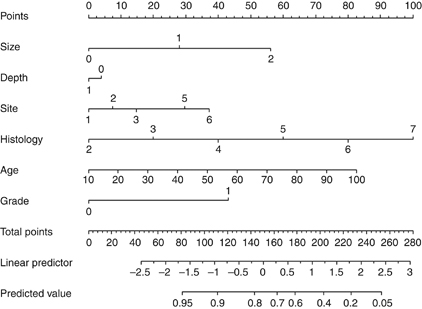
\includegraphics[width=.8\linewidth]{figs/080-kattan.jpeg}
  \caption{Pooperativni nomogram (Kattan in sod. (1999) {\em Journal of Clinical Oncology} 17(5).) za napoved 12-letne verjetnosti preživetja brez ponovitve raka prostate po radikalni prostatektomiji. Nomogram uporabimo tako, da za vsako vrednost klinične značilke odčitamo pripadajoče število točk na zgornji lestvici, točke seštejemo, nato pa skupno vsoto na spodnji lestvici preslikamo v napovedano verjetnost. Nomogram nam poleg pomoči za napoved grafično predstavi tudi pomembnost posameznih značilk.}
  \label{fig:kattan}
\end{figure}

V tem poglavju si bomo ogledali vrsto napovednih modelov, ki jih lahko učinkovito predstavimo z nomogrami, zlasti v njihovi preprostejši obliki, kot jo ponazarja Kattanov nomogram. Začnemo z linearno regresijo, nato pa preidemo na širši razred modelov, ki kljub morebitni nelinearni transformaciji ohranjajo linearno strukturo v parametrih, ter raziščemo, v kolikšni meri jih lahko enotno obravnavamo v okviru posplošenih linearnih modelov. Čeprav nomografija kot disciplina ponuja bistveno širši nabor pristopov in konstrukcij, se njena sodobna uporaba pri napovednih modelih večinoma omejuje prav na takšne, pregledne in interpretabilne oblike, ki omogočajo neposredno povezavo med vhodnimi značilkami in končno napovedjo, kot je razvidno na sliki~\ref{fig:kattan}.

\section{Nomogram za model linearne regresije}

Tole bo kar precej enostavno. Linearna regresija je utežena vsota. Vsak del utežene vsote lahko obravnavamo kot točke, ki se na koncu seštejejo in pretvorijo v končno napoved. Točkovanje lahko poenostavimo tako, da so točke celoštevilske in jih je na koncu enostavneje sešteti, vendar potrebujemo pretvorbo v končno veličino, ki pa je linearna. Primer takega nomograma prikazuje slika~\ref{fig:bodyfat} z nam že znanim primerom izračuna deleža telesnih maščob.

\begin{figure}[ht]
\centering
\includegraphics[width=\linewidth]{figs/080-lin.pdf}
\caption{Nomogram linearne regresije za izračun deleža telesnih maščob (t. i. {\em body fat Brozek}). Iz grafa je jasno razvidno, da je ključna spremenljivka obseg trebuha, veliko manjšo vlogo ima teža, medtem ko je vpliv starosti in mer bicepsa skoraj zanemarljiv. Vpliv začetne vrednosti funkcije smo upoštevali pri pretvorbi zbranih točk v vrednost razreda.}
\label{fig:bodyfat}
\end{figure}

Z nomogramom smo model grafično predstavili tako, da ga lahko sedaj uporabljamo tudi brez računalnika, zgolj z odčitavanjem in seštevanjem točk. Takšen prikaz obenem jasno poudari pomen posameznih značilk oziroma njihovo ``moč'' v modelu, saj se njihov vpliv neposredno odraža v razponu točk, ki jih prispevajo k skupni napovedi.

Postavlja se vprašanje, ali obstajajo tudi drugi, podobno enostavni modeli za nekoliko drugačne napovedne naloge, torej takšni, pri katerih značilke prav tako povežemo z uteženo vsoto, nato pa dobljeno vrednost preoblikujemo z ustrezno (nelinearno) povezovalno funkcijo, tako da lahko modeliramo tudi diskretne ali kako drugače omejene ciljne spremenljivke. V nadaljevanju začnemo s primerom takšnega modela, ki ga bomo uporabili za razvrščanje, nato pa se vprašamo, ali so tovrstne razširitve dovolj splošne za širši razred modelov, kaj pri njih pravzaprav predpostavimo, od kod izhajajo njihove kriterijske funkcije in ali gre pri tem za zanimiv razred modelov s skupnimi lastnostmi.

\section{Uvod v logistično regresijo}

Začnimo z (izmišljenim) primerom. V tabeli s slike~\ref{tab:bled} so zbrani kopalci na Bledu, ki smo jih vprašali, koliko ur na teden se ukvarjajo s športom in koliko ur so prejšnjo noč spali. Zabeležili smo tudi, ali so v dnevu intervjuvanja uspeli odplavati na otok. Ta je od bližnjega kopališča oddaljen več kot pol kilometra v eni smeri, zato je plavanje na otok in nazaj kar zalogaj, ki ne bi bil ravno primeren za slabše kopalce. Cilj je razviti aplikacijo, ki bi kopalcem svetovala, seveda glede na fizično pripravljenost in spočitost, ali naj se napotijo na tak podvig. Aplikacija seveda potrebuje napovedni model, tega pa lahko zgradimo iz naših podatkov.



\begin{marginfigure}
\caption{Primer klasifikacijskih podatkov z meta atributum, neodvisnima spremenljivkama in razredom (Otok).}
\label{tab:bled}
\footnotesize
\centering
\begin{tabular}{lccc}
\toprule
Ime & Vadba & Spanje & Otok \\
\midrule
Alenka     & 7  & 8 & 1 \\
Ana        & 2  & 8 & 0 \\
Andrej     & 5  & 5 & 0 \\
Blaž       & 5  & 9 & 1 \\
Boštjan    & 7  & 5 & 0 \\
Goran      & 12 & 6 & 1 \\
Gregor     & 10 & 9 & 1 \\
Helena     & 4  & 9 & 1 \\
Irena      & 9  & 3 & 0 \\
Janez      & 5  & 6 & 0 \\
Jure       & 8  & 4 & 0 \\
Katarina   & 4  & 3 & 0 \\
Klara      & 3  & 9 & 1 \\
Luka       & 5  & 4 & 0 \\
Maja       & 9  & 6 & 0 \\
Marko      & 4  & 7 & 0 \\
Matej      & 4  & 8 & 1 \\
Miha       & 6  & 4 & 0 \\
Mojca      & 11 & 5 & 1 \\
Nika       & 2  & 5 & 0 \\
Nina       & 8  & 6 & 1 \\
Petra      & 3  & 6 & 0 \\
Polona     & 9  & 8 & 1 \\
Rok        & 10 & 6 & 1 \\
Sara       & 6  & 7 & 1 \\
Sašo       & 10 & 7 & 1 \\
Sebastjan  & 12 & 5 & 1 \\
Tatjana    & 12 & 9 & 1 \\
Tjaša      & 11 & 3 & 0 \\
Tomaz      & 12 & 5 & 1 \\
\bottomrule
\end{tabular}
\end{marginfigure}

Ker so podatki dvodimenzionalni, jih je najbolje izrisati v razsevnem diagramu. Označimo tudi razred. Že prvi pogled na izris kaže, da je morda mogoče dobre plavalce in tiste, ki se bolj kopajo, ločiti s črto oziroma odločitveno mejo. Ta je linearna, zato jo lahko zapišemo kot $x^T\theta = 0$. Izris vključuje tudi tri nove obiskovalce: Saro, Martina in Leona. Kateremu izmed njih bo naša aplikacija oziroma model svetovala, da lahko odplava do otoka in priplava nazaj?

Sara je na strani plavalcev. Je daleč od odločitvene meje ki loči med obema razredoma. Prav gotovo lahko plava do otoka in nazaj. Martin je zelo na drugi strani, nikakor naj se ne oddalji od obale. Leon je, kar se tiče odločitvene meje, na strani plavalcev, a za las. Svetovati mu da naj poskusi plavati do otoka bi bilo zelo narobe. Naš problem je sicer klasifikacijski, želimo napovedati enega od dveh možnih razredov, a bolje bi bilo to narediti previdno, z uporabo verjetnosti. Ker je Sara zelo oddaljena od odločitvene meje, je prav gotovo kandidatka za odhod na otok, Martin nikakor ne, Leon pa je nekje na maje, njegova verjetnos ``plavalnega'' razreda je okoli 50\%.

Postaja nam jasno: oddaljenost od odločitvene meje moramo pretvoriti v verjetnosti. Kar seveda ne bo problem. Linearna kombinacija $z = x^T\theta$ je pravzaprav proporcionalna oddaljenosti od premice, ki jo določajo parametri $\theta$. Za pretvorbo lahko uporabimo funkcijo, katere zaloga vrednosti je med $0$ in $1$. Primer take funkcije je sigmoida $\sigma(z)$, naša verjetnost pa je potem
\[
P(y = 1 \mid x) = \sigma(z) = \frac{1}{1 + e^{-z}}.
\]

\begin{figure}[ht]
    \centering
    \includegraphics[width=0.8\linewidth]{figs/080-bled-scatter.pdf }
    \caption{Učni podatki, možna ločitvena meja med razredoma, in novi (imenovani) primeri, ki jih moramo še razvrstiti.}
    \label{fig:bled}
\end{figure}

\begin{marginfigure}
    \centering
    \includegraphics[width=\linewidth]{figs/080-sigmoid.pdf}
    \caption{Sigmoidna funkcija.}
    \label{fig:sigmoida}
\end{marginfigure}
%
Odločitvena meja s slike~\ref{fig:bled} ima parametre parametre $\theta_0=-15.6$, $\theta_1=0.8$ in $\theta_2=1.6$, zato lahko odločitveno enačbo za oddaljenost od te meje zapišemo kot
\[
z = -15.6 + 0.8 \cdot \text{vadba} + 1.6 \cdot \text{spanje}.
\]
Za nove primere dobimo: Sara ima $z=5.5$ in $P(\text{otok}=1)\approx 1.0$, zato je zelo primerna kandidatka za plavanje do otoka; Martin ima $z=-6.7$ in $P(\text{otok}=1)\approx 0.0$, zato mu to odsvetujemo; Leon pa ima $z=0.6$ in $P(\text{otok}=1)\approx 0.6$, kar pomeni, da je blizu odločitvene meje in je odločitev precej negotova.

Dobljeni model lahko predstavimo z nomogramom (slika~\ref{fig:bled-nnomogram}).

\begin{figure}[ht]
    \centering
    \includegraphics[width=0.8\linewidth]{figs/080-bled-nomogram.pdf }
    \caption{Nomogram za napovedovanja verjentosti plavanja na Blejski otok.}
    \label{fig:bled-nnomogram}
\end{figure}

Dobljeni model lahko predstavimo z nomogramom (slika~\ref{fig:bled-nnomogram}). Pri tem vsakemu vhodnemu atributu (vadba, spanje) priredimo svojo lestvico, na kateri posamezna vrednost atributa prispeva določeno število točk, sorazmerno z utežjo v linearni kombinaciji. Te točke nato seštejemo v skupni rezultat, ki ustreza vrednosti linearnega napovednega dela $z = x^T\theta$. Ker pa nas pri logistični regresiji ne zanima neposredno $z$, temveč verjetnost, se v naslednjem koraku skupni rezultat preslika še skozi sigmoidno funkcijo, kar v nomogramu običajno ponazorimo z dodatno, nelinearno lestvico na dnu grafa. Tako dobimo celovit vizualni pripomoček, ki omogoča, da brez eksplicitnega računanja najprej ocenimo prispevek posameznih dejavnikov, nato njihovo vsoto in končno še pripadajočo verjetnost razreda. Takšna predstavitev je posebej uporabna v praksi, saj združuje interpretabilnost linearnega modela z intuitivnim razumevanjem verjetnosti: uporabnik lahko neposredno vidi, kako sprememba ene spremenljivke vpliva na končni izid, hkrati pa ohrani občutek za negotovost napovedi, zlasti v bližini odločitvene meje.

Model, ki smo ga precej na hitro in morda malo površno uvedli na našem primeru se imenuje logistična regresija. Pomembno je, da tako kot linearna regresija tudi ta model uporablja linearno kombinacijo neodvisnih spremenljivk, katere rezultat pa tokrat, čisto zato, da lahko vrnemo verjetnosti, transformiramo z sigmoidno funkcijo. A postavlja se vprašanje: kako se sploh naučimo ``pravih'' parametrov našega modela, toej vektorja $\theta$? Kakšno kriterijsko funkcijo za to optimiziramo? Iz kakšnih predpostavk ta izhaja? Poznamo poleg linearne in logistične regresije še kakšne druge modele te vrste? In končno, je tudi to moč uporabiti strojno odvajanje in gradientni sestop za učenje modela?

Čas je za malce teorije.

\section{Eksponentna družina porazdelitev}

Od kod torej izhajajo modeli, kot sta linearna in logistična regresija? Kakšne predpostavke sploh pri tem naredimo o podatkih? Uberemo podoben pristop kot ga že poznamo pri linearni regresiji: namesto, da bi si izmislili kriterijsko funkcijo (npr. vsota kvadratov napak na učni množici), bomo izhajali iz verjetnostnega modela, torej modela, ki generira podatke v učno množico, in iz te predpostavke izpeljali kriterijsko funkcijo.

Razred porazdelitev, ki se za naš namen izkaže še posebej uporaben, je \emph{eksponentna družina}. Porazdelitev spada v to družino, če njeno verjetnostno funkcijo (ali gostoto) za spremenljivko $y$ lahko zapišemo v obliki
\[
p(y \mid \eta) = h(y)\,\exp\left(\eta\,T(y) - A(\eta)\right),
\]
kjer je $\eta = \eta(\theta)$ naravni parameter, $T(y)$ zadostna statistika,
$A(\eta)$ normalizacijska funkcija, $h(y)$ pa od parametra neodvisen del. Torej:
\begin{itemize}
  \item $\theta$ so parametri modela,
  \item $\eta$ je naravni parameter porazdelitve; v posplošenih linearnih modelih predpostavimo, da velja $\eta(x)=x^T\theta$, zato je model linearen v~$\eta$,
%
\marginnote{
Izpeljimo povezavo med $A(\eta)$ in pričakovano vrednostjo naključne spremenljivke $y$. Ker je integral gostote verjetnosti po definiciji enak 1, velja
\[
\int h(y)\,\exp\big(\eta T(y) - A(\eta)\big)\,dy = 1.
\]
Odvajanje zgornje enačbe po $\eta$ da
\[
\mathbb{E}[T(y)] - A'(\eta) = 0,
\]
zato
\[
\mathbb{E}[T(y)] = A'(\eta).
\]
V številnih primerih velja $T(y)=y$, zato je tedaj $A'(\eta)$ enak pričakovani vrednosti naključne spremenljivke $y$.
}
%
  \item $A(\eta)$ je normalizacijska funkcija, za katero velja $\mathbb{E}[T(y)] = A'(\eta)$,
  \item $\mu(x)=\mathbb{E}[T(y)\mid x]$ je povezana z $\eta$ prek zveze $\mu = A'(\eta)$; v primeru $T(y)=y$ to ustreza $\mathbb{E}[y \mid x]$.
\end{itemize}

Ker nas bo pri strojnem učenju zanimal logaritem verjetja, je smiselno izraz za verjetnostno funkcijo za eksponentno družino logaritmirati:
\[
\log p(y \mid \eta) = \eta T(y) - A(\eta) + \log h(y).
\]

V razdelkih, ki sledijo, si bomo ogledali tri primere porazdelitev,
ki sodijo v to družino in iz katerih izhajajo linearna, logistična
in Poissonova regresija. Vsak primer bomo analizirali v naslednjih korakih:

\begin{enumerate}
\item \textbf{Privzeta porazdelitev}: zapišemo verjetnostno porazdelitev
      za naključno spremenljivko $y$ (oziroma njen logaritem) ter jo
      preuredimo v obliko eksponentne družine,

\item \textbf{Pričakovana vrednost}: izračunamo pričakovano vrednost
      \[
      \mu(x)=\mathbb{E}[y\mid x],
      \]
      in preverimo, da se ujema z zvezo $\mu = A'(\eta)$. Ta korak bi
      sicer lahko pri spodnji obravnavi posameznih modelov tudi
      izpustili, vendar se ga splača izvesti, saj nam pomaga bolje
      razumeti entitete, ki nastopajo v eksponentni družini, hkrati pa
      se ob tem spomnimo tudi izrazov za pričakovano vrednost pri
      posameznih porazdelitvah.

\item \textbf{Povezava med povprečjem in linearnim napovednikom}: 
      v tem poglavju se bomo omejili na modele, pri katerih naravni
      parameter porazdelitve določimo z linearno kombinacijo značilk,
      torej
      \[
      \eta(x)=x^T\theta.
      \]
      Nato bomo poiskali, kako je povprečna vrednost
      \[
      \mu(x)=\mathbb{E}[y\mid x]
      \]
      povezana s tem linearnim napovednikom. To zvezo opišemo s
      povezovalno funkcijo $g$, za katero velja
      \[
      g(\mu(x)) = x^T\theta.
      \]

\item \textbf{Verjetje}: zapišemo logaritemsko verjetje, iz katerega dobimo kriterijsko funkcijo za učenje modela. Ker smo v prvi točki že zapisali verjetnostno funkcijo ciljne spremenljivke, je ta korak skoraj nepotreben, a ne škodi zapisati kriterijsko funkcijo, ki jo bomo optimizirali pri učenju modela, da bo pri roki za implementacijo.
\end{enumerate}

\subsection{Verjetje in učenje modela}

Tu naj samo spomnimo, da bomo za določitev parametrov modela potrebovali kriterijsko funkcijo, za to pa potrebujemo verjetje oziroma njegov logaritem. Pravzaprav imamo za to že vse pripravljeno. Predpostavimo, da so učni primeri med seboj neodvisni, in ko se še odločimo za ciljno  porazdelitev razredov, lahko zapišemo verjetje za učne podatke
\[
p(\mathbf{y} \mid X, \theta) = \prod_{i=1}^n p(y_i \mid x_i, \theta).
\]
Za učenje parametrov maksimiziramo logaritemsko verjetje
\[
\ell(\theta) = \sum_{i=1}^n \log p(y_i \mid x_i, \theta),
\]
kar je ekvivalentno minimizaciji negativnega log-verjetja, ki ga lahko razumemo kot kriterijsko funkcijo.

Na tej točki postane povezava s strojnim učenjem očitna: različne izbire porazdelitev vodijo do različnih kriterijskih funkcij, optimizacija pa poteka enako, npr.\ z gradientnim sestopom.

\section{Linearna regresija je poseben primer eksponentne družine}

Na uporabnost eksponentne družine porazdelitev moramo šele pokazati.
Pričnimo z najpreprostejšim primerom: linearno regresijo, ki jo bomo
obdelali po zgoraj opisanih korakih.

\begin{enumerate}

\item \textbf{Privzeta porazdelitev.}
Predpostavimo, da je izhodna spremenljivka pri danih značilkah $x$
normalno porazdeljena:
\[
y \mid x \sim \mathcal{N}(\mu(x), \sigma^2),
\]
z gostoto
\[
p(y \mid x) = \frac{1}{\sqrt{2\pi\sigma^2}}
\exp\!\left(-\frac{(y - \mu(x))^2}{2\sigma^2}\right).
\]

Logaritem gostote je
\[
\log p(y \mid x) =
-\frac{(y - \mu)^2}{2\sigma^2}
- \frac{1}{2}\log(2\pi\sigma^2),
\]
kar po razvoju da
\[
\log p(y \mid x)
= \frac{\mu}{\sigma^2} y
- \frac{\mu^2}{2\sigma^2}
- \frac{y^2}{2\sigma^2}
- \frac{1}{2}\log(2\pi\sigma^2).
\]

To je oblike eksponentne družine
\[
\log p(y \mid \eta)
= \eta\,T(y) - A(\eta) + \log h(y),
\]
kjer prepoznamo
\[
T(y)=y, \qquad
\eta = \frac{\mu}{\sigma^2},
\]
\[
A(\eta) = \frac{\sigma^2}{2}\eta^2, \qquad
\log h(y)= -\frac{y^2}{2\sigma^2} - \frac{1}{2}\log(2\pi\sigma^2).
\]

\item \textbf{Pričakovana vrednost.}
Za eksponentno družino velja $\mathbb{E}[T(y)] = A'(\eta)$, zato
\[
\mathbb{E}[y \mid x] = A'(\eta).
\]

Ker je
\[
A(\eta) = \frac{\sigma^2}{2}\eta^2,
\]
dobimo
\[
A'(\eta) = \sigma^2 \eta.
\]

Ker velja $\eta = \frac{\mu}{\sigma^2}$, sledi
\[
A'(\eta) = \mu,
\]
torej
\[
\mu(x) = \mathbb{E}[y \mid x].
\]

\item \textbf{Povezava med $\mu$ in linearnim napovednikom.}
Iz zveze $\eta = \frac{\mu}{\sigma^2}$ (pri konstantni varianci)
sledi $\eta \propto \mu$, zato lahko $\eta$ obravnavamo kot $\mu$.
Če predpostavimo
\[
\eta(x) = x^T\theta,
\]
dobimo
\[
\mu(x) = x^T\theta,
\]
torej je povezovalna funkcija identiteta.

\item \textbf{Verjetje.}
Logaritemsko verjetje za en primer je
\[
\log p(y \mid x, \theta) =
-\frac{1}{2\sigma^2}(y - x^T\theta)^2
- \frac{1}{2}\log(2\pi\sigma^2).
\]

Logaritemsko verjetje na učni množici, kjer predpostavimo neodvisnost učnih primerov, je
\[
\ell(\theta)
=
\sum_{i=1}^n
\left[
-\frac{1}{2\sigma^2}(y_i - x_i^T\theta)^2
- \frac{1}{2}\log(2\pi\sigma^2)
\right].
\]

Drugi člen ne zavisi od $\theta$, zato ga pri optimizaciji lahko
zanemarimo. Parametre modela določimo kot
\[
\theta^*
=
\arg\min_\theta L(\theta)
=
\arg\min_\theta
\sum_{i=1}^n (y_i - x_i^T \theta)^2.
\]

\end{enumerate}


\section{Tudi logistična regresija je primer eksponentne družine}

Podobno kot pri linearni regresiji bomo tudi logistično regresijo
analizirali v okviru eksponentne družine porazdelitev.

\begin{enumerate}

\item \textbf{Privzeta porazdelitev.}
Pri binarni klasifikaciji predpostavimo, da ciljna spremenljivka
pri danih značilkah $x$ sledi Bernoullijevi porazdelitvi:
\[
y \mid x \sim \mathrm{Bernoulli}(p(x)),
\]
kjer velja $y \in \{0,1\}$ in
\[
P(y=1 \mid x) = p(x), \qquad P(y=0 \mid x) = 1 - p(x).
\]

Gostoto zapišemo kot
\[
p(y \mid x) = p^y (1-p)^{1-y}.
\]

Logaritem gostote je
\[
\log p(y \mid x) = y \log p + (1-y)\log(1-p),
\]
kar preuredimo v
\[
\log p(y \mid x)
= y \log \frac{p}{1-p} + \log(1-p).
\]

To je oblike eksponentne družine
\[
\log p(y \mid \eta)
= \eta\,T(y) - A(\eta) + \log h(y),
\]
kjer prepoznamo
\[
T(y)=y, \qquad
\eta = \log\frac{p}{1-p}.
\]

Funkcijo $A$ izrazimo kot funkcijo $\eta$:
\[
A(\eta) = \log(1 + e^\eta), \qquad h(y)=1.
\]

\item \textbf{Pričakovana vrednost.} Ker je
\[
A(\eta) = \log(1 + e^\eta),
\]
dobimo
\[
A'(\eta) = \frac{e^\eta}{1 + e^\eta}.
\]

Ker velja $\eta = \log\frac{p}{1-p}$, sledi $e^\eta = \frac{p}{1-p}$ in zato
\[
A'(\eta) = \mathbb{E}[y \mid x] = p.
\]

\item \textbf{Povezava med $\mu$ in linearnim napovednikom.}
Naravni parameter je
\[
\eta = \log \frac{p}{1-p}.
\]

Ker je $\mu = p$, dobimo povezovalno funkcijo (logit)
\[
g(\mu(x)) = \log \frac{\mu(x)}{1-\mu(x)}.
\]

Če predpostavimo
\[
\eta(x) = x^T\theta,
\]
sledi
\[
\log \frac{p(x)}{1-p(x)} = x^T\theta,
\]
od koder dobimo
\[
p(x) = \frac{1}{1 + e^{-x^T\theta}}.
\]

\item \textbf{Verjetje.}
Logaritemsko verjetje za en primer je
\[
\log p(y \mid x, \theta)
= y \log p(x) + (1-y)\log(1-p(x)).
\]

Če predpostavimo neodvisnost primerov v učni množici, je logaritemsko verjetje:
\[
\ell(\theta)
= \sum_{i=1}^n \left[
y_i \log p(x_i) + (1-y_i)\log(1-p(x_i))
\right].
\]

Parametre modela določimo z minimizacijo negativnega log-verjetja:
\[
\theta^*
=
\arg\min_\theta
\left(
-\sum_{i=1}^n \left[
y_i \log p(x_i) + (1-y_i)\log(1-p(x_i))
\right]
\right),
\]
kar ustreza kriterijski funkciji, ki jo poznamo kot križna entropija.

\end{enumerate}

\section{Poissonova regresija}

Pri številnih praktičnih problemih nas ne zanima napoved zvezne količine ali verjetnosti, temveč število dogodkov v nekem časovnem ali prostorskem intervalu. Takšni primeri so na primer število prihodov strank v trgovino na uro, število prometnih nesreč na določenem odseku ceste, število klicev v klicni center ali število pojavitev določene bolezni v populaciji. Za takšne podatke je značilno, da so nenegativna cela števila in pogosto asimetrično porazdeljeni, zato linearna regresija ni primerna: lahko bi napovedovala negativne vrednosti, poleg tega pa predpostavlja konstantno varianco, kar pri štetjih običajno ne drži (varianca pogosto narašča s povprečjem). V takih primerih je smiselno uporabiti model, ki upošteva naravo podatkov, zato uporabimo Poissonovo porazdelitev, ki je v splošnem
\[
p(y) = \frac{\lambda^y e^{-\lambda}}{y!},
\]
kjer je parameter $\lambda > 0$ intenziteta procesa, torej pričakovano število dogodkov v danem intervalu, za katerega velja
\[
\mathbb{E}[y] = \lambda.
\]

\begin{enumerate}

\item \textbf{Privzeta porazdelitev.}
Predpostavimo, da ciljna spremenljivka pri danih značilkah $x$ sledi
Poissonovi porazdelitvi:
\[
y \mid x \sim \mathrm{Poisson}(\lambda(x)),
\]
kjer velja $y \in \{0,1,2,\dots\}$ in
\[
p(y \mid x) = \frac{\lambda^y e^{-\lambda}}{y!}.
\]
Parameter $\lambda(x) > 0$ predstavlja intenziteto oziroma pričakovano število dogodkov pri danih značilkah $x$, zato velja
\[
\mu(x) = \mathbb{E}[y \mid x] = \lambda(x).
\]

Logaritem gostote je
\[
\log p(y \mid x)
= y \log \lambda - \lambda - \log(y!).
\]
in če ga primerjamo z obliko eksponentne družine
\[
\log p(y \mid \eta)
= \eta\,T(y) - A(\eta) + \log h(y),
\]
lahko prepoznamo
\[
T(y)=y, \qquad
\eta = \log \lambda.
\]

Funkcijo $A$ izrazimo kot funkcijo $\eta$:
\[
A(\eta) = e^\eta, \qquad
h(y) = \frac{1}{y!}.
\]

\item \textbf{Pričakovana vrednost.} Ker je
\[
A(\eta) = e^\eta,
\]
dobimo
\[
A'(\eta) = e^\eta.
\]

Ker velja $\eta = \log \lambda$, sledi $e^\eta = \lambda$ in zato
\[
A'(\eta) = \lambda.
\]

Torej
\[
\mu(x) = \mathbb{E}[y \mid x] = \lambda(x).
\]

\item \textbf{Povezava med $\mu$ in linearnim napovednikom.}
Naravni parameter je
\[
\eta = \log \lambda.
\]

Ker je $\mu = \lambda$, dobimo povezovalno funkcijo (log)
\[
g(\mu(x)) = \log \mu(x).
\]

Če predpostavimo
\[
\eta(x) = x^T\theta,
\]
sledi
\[
\log \lambda(x) = x^T\theta,
\]
od koder dobimo
\[
\lambda(x) = e^{x^T\theta}.
\]

\item \textbf{Verjetje.}
Logaritemsko verjetje za en primer je
\[
\log p(y \mid x, \theta)
= y x^T\theta - e^{x^T\theta} - \log(y!).
\]

Logaritemsko verjetje na učni množici, kjer predpostavimo neodvisnost primerov, je:
\[
\ell(\theta)
= \sum_{i=1}^n \left[
y_i x_i^T\theta - e^{x_i^T\theta} - \log(y_i!)
\right].
\]

Ker člen $\log(y_i!)$ ne zavisi od $\theta$, ga pri optimizaciji
lahko zanemarimo. Parametre modela zato določimo z minimizacijo
negativnega log-verjetja:
\[
\theta^*
=
\arg\min_\theta
\sum_{i=1}^n \left[
e^{x_i^T\theta} - y_i x_i^T\theta
\right].
\]

\end{enumerate}

\begin{table}[htb]
\centering
\small
\renewcommand{\arraystretch}{1.4}
\begin{tabularx}{\linewidth}{X X X X}
\toprule
Porazdelitev & Tip izhoda & Kaj modeliramo & Tipične uporabe \\
\midrule
Normalna & zvezna vrednost & simetrične zvezne meritve & linearna regresija \\
Bernoullijeva & 0/1 & verjetnost dogodka & klasifikacija \\
Poissonova & cela števila & število dogodkov & prihodi, klici, nesreče \\
Gamma & pozitivna zvezna vrednost & trajanje ali strošek & čakalni časi, zavarovanja \\
Negativna binomska & cela števila & preveč razpršena štetja & epidemiologija, biologija \\
\bottomrule
\end{tabularx}
\caption{Primeri porazdelitev v posplošenih linearnih modelih.}
\label{tab:glm}
\end{table}

\section{Kaj pa ostale porazdelitve iz eksponentne družine?}

Zgoraj opisane porazdelitve nikakor niso edine, ki jih uporabljamo pri gradnji posplošenih linearnih modelov. Poleg normalne, Bernoullijeve in Poissonove porazdelitve poznamo še vrsto drugih modelov iz eksponentne družine, ki so primerni za različne tipe podatkov in napovednih nalog. Posebej uporabne so takrat, ko ciljna spremenljivka ni zvezna, ni simetrično porazdeljena ali pa je omejena na pozitivne vrednosti oziroma števila dogodkov.

Tabela~\ref{tab:glm} podaja nekaj najpogosteje uporabljenih porazdelitev v posplošenih linearnih modelih ter tipične probleme, pri katerih jih uporabimo. Poleg treh zgoraj podrobneje obravnavanih smo vključili še porazdelitev Gamma, ki jo pogosto uporabljamo za modeliranje pozitivnih zveznih količin, kot so trajanja, čakalni časi ali stroški, ter negativno binomsko porazdelitev, ki je posebej uporabna pri modeliranju štetij z veliko razpršenostjo podatkov.

\section{Primer implementacije}

Zgornje besedilo je vključevalo veliko teorije in malo primerov. Za (bolj računalniški) premor implementirajmo logistično regresijo. Tako kot pri linearni regresiji iz prejšnjega poglavju, začnemo s razredom, ki razvije kriterijsko funkcijo nad vhodnimi podatki.

\vspace*{3mm}
\begin{lstlisting}
class LogReg:
    def __init__(self, n_inputs, reg=None, reg_strength=0.0):
        self.weights = 
          [Value(random.uniform(-1, 1), label=f"w{i}")
           for i in range(n_inputs)]
        self.b = Value(0.0, label="b")
        self.reg = reg
        self.reg_strength = reg_strength

    def linear(self, x):
        return sum(w * xi for w, xi in zip(self.weights, x)) + self.b

    def __call__(self, x):
        return self.linear(x).sigmoid()

    def parameters(self):
        return self.weights + [self.b]

    def loss(self, xs, ys):
        eps = 1e-8
        losses = []
        for x, y in zip(xs, ys):
            yhat = self(x)
            y_val = Value(float(y))
            term = -(y_val * (yhat + eps).log() + \
              (1 - y_val) * (1 - yhat + eps).log())
            losses.append(term)
        data_loss = sum(losses) / Value(len(xs))

        if self.reg == "l2" and self.reg_strength > 0:
            l2_penalty = self.reg_strength * sum(w * w for w in self.weights)
            return data_loss + l2_penalty
        return data_loss

    def __repr__(self):
        weights_str = ", ".join(f"w{i}={w.data:.3f}" \
          for i, w in enumerate(self.weights))
        return f"LogReg({weights_str}, b={self.b.data:.3f})"
\end{lstlisting}

Koda implementira logistično regresijo v duhu posplošenih linearnih modelov.
%
\marginnote{Podoben razred bi lahko zapisali tudi za Poissonovo regresijo ali druge posplošene linearne modele. Pravzaprav bi bilo smiselno definirati splošen razred za take modele, ki implementira skupno strukturo (linearni napovednik in učenje), posamezni modeli pa bi podedovali le ustrezno povezovalno funkcijo in kriterijsko funkcijo. To posplošitev prepuščamo bralcu.}
%
Metoda \texttt{linear} izračuna linearni napovednik $x^T\theta$, metoda \texttt{\_\_call\_\_} pa ga preslika skozi sigmoidno funkcijo in tako vrne verjetnost razreda. Funkcija \texttt{loss} ustreza negativnemu log-verjetju (križni entropiji), ki smo ga izpeljali zgoraj, in jo minimiziramo pri učenju modela. V implementacijo smo vključili tudi možnost regularizacije. Če izberemo L2-regularizacijo, se kriterijski funkciji prišteje kazenski člen, ki zavira prevelike vrednosti uteži in tako pomaga preprečevati prenaučenost modela.

Sledi koda za učenje, kjer smo kot funkcijo za učenje uporabili kar to že razvito in zapisano v knjižnica \texttt{agrad}:

\marginnote{Podatki za naš primer so na voljo na 
\href{https://file.biolab.si/datasets/bled-plavanje.xlsx}
{\texttt{bled-plavanje.xlsx}}.
}
%
\vspace*{3mm}
\begin{lstlisting}
df = pd.read_excel("bled-plavanje.xlsx")
feature_names = ["vadba", "spanje"]
xs = df[feature_names].values.tolist()
ys = df["otok"].astype(int).tolist()

print(df[["vadba", "spanje", "otok"]].head().to_string(index=False))

model = LogReg(n_inputs=len(feature_names), reg="l2", reg_strength=0.01)
model = train(model, xs, ys, learning_rate=0.1, n_epochs=10000, batch_size=None)
\end{lstlisting}

Optimizacija konvergira sorazmerno hitro, pridobljeni parametri pa se dobro ujemajo s tistimi iz slike~\ref{fig:bled}.

\vspace*{3mm}
\begin{lstlisting}
>>> model
LogReg(w0=0.756, w1=1.566, b=-14.822)
\end{lstlisting}

% \section{Multinomna logistična regresija}

% Logistična regresija, kot smo jo uvedli zgoraj, obravnava binarni, torej dvovrednostni klasifikacijski problem. A tipično se pri klasifikaciji s problemi, kjer je razredov več. Pri klasifikaciji slik želimo na primer določiti, kateri predmet je na sliki, pri obdelavi besedil pa napovedujemo temo dokumenta ali naslednji zlog ali besedo v stavku. V takih primerih je število možnih izhodov (veliko) večje od dveh, zato potrebujemo modele, ki znajo napovedovati porazdelitev verjetnosti čez več razredov. Eden najpogosteje uporabljenih modelov za ta namen je multinomna logistična regresija, znana tudi kot \emph{softmax regresija}, ki se zelo pogosto pojavi kot izhodna plast nevronskih mrež.

% Naj bo ciljna spremenljivka $y \in \{1,2,\dots,m\}$, kjer je $m$ število razredov. Za vsak razred $j$ definiramo linearni napovednik
% \[
% z_j = x^T \theta_j.
% \]

% Ker želimo dobiti verjetnosti, ki so nenegativne in seštejejo v~1, uporabimo funkcijo
% \[
% P(y = j \mid x) = \frac{e^{z_j}}{\sum_{l=1}^m e^{z_l}},
% \]
% ki ji pravimo \emph{softmax}. Ta funkcija preslika vektor realnih vrednosti $(z_1,\dots,z_m)$ v verjetnostni vektor.

% Model ni enolično določen, saj lahko vsem $z_j$ prištejemo isto konstanto, ne da bi se verjetnosti spremenile. Zato običajno en razred izberemo kot referenčni razred in njegov linearni napovednik nastavimo na nič:
% \[
% z_m = 0.
% \]

% Model ima tako $(m-1)$ vektorjev parametrov. Multinomna logistična regresija je posplošeni linearni model, kjer ciljna spremenljivka sledi kategorični porazdelitvi, je linearni napovednik $z_j = x^T \theta_j$, je povezovalna funkcija posplošeni logit, katere inverz je funkcija softmax.

% Model lahko zapišemo tudi kot
% \[
% y \mid x \sim \mathrm{Categorical}(p_1(x), \dots, p_m(x)),
% \]
% kjer velja
% \[
% p_j(x) = \frac{e^{x^T \theta_j}}{\sum_{l=1}^m e^{x^T \theta_l}}.
% \]

% Če imamo le dva razreda ($m=2$), se softmax poenostavi v sigmoidno funkcijo in dobimo običajno logistično regresijo. 

% Parametre modela ocenimo z maksimizacijo logaritemskega verjetja
% \[
% \ell(\theta) = \sum_{i=1}^n \log P(y_i \mid x_i),
% \]
% kar vodi do kriterijske funkcije, ki jo poznamo kot večrazredno križno entropijo. Tako kot pri logistični regresiji analitične oblike rešitve ni, zato parametre ocenjujemo numerično, npr.\ z gradientnim sestopom.

\section{Posplošeni linearni modeli in nomogrami danes}

Posplošeni linearni modeli se v praksi zelo pogosto uporabljajo, zlasti v medicini, epidemiologiji, ekonomiji in drugih aplikativnih vedah. Združujejo preprostost, interpretabilnost in dovolj veliko izrazno moč, da jih lahko uspešno uporabimo pri številnih napovednih nalogah. Pomembni so tudi zato, ker jih lahko zelo učinkovito predstavimo z nomogrami. Njihova struktura — linearna kombinacija značilk in enostavna nelinearna preslikava — omogoča neposredno pretvorbo modela v grafično orodje, kjer posamezne spremenljivke prispevajo točke, te pa vodijo do končne napovedi.

Pomembni so tudi pri oblikovanju sodobne umetne inteligence. Izhodne plasti nevronskih mrež so praviloma posplošeni linearni modeli: pri regresiji linearni model, pri dvorazredni klasifikaciji logistična regresija, pri večrazredni klasifikaciji pa multinomna logistična regresija (softmax). Podobno velja za notranje enote nevronskih mrež: vsaka najprej izračuna linearno kombinacijo vhodov, nato pa jo preslika skozi nelinearno funkcijo, kot je logistična funkcija ali njene preprostejše alternative (npr.\ ReLU). O tem več v naslednjih poglavjih.